\documentclass[10pt, landscape]{article}
\usepackage[scaled=0.92]{helvet}
\usepackage{calc}
\usepackage{multicol}
\usepackage{ifthen}
\usepackage[a4paper,margin=3mm,landscape]{geometry}
\usepackage{amsmath,amsthm,amsfonts,amssymb}
\usepackage{color,graphicx,overpic}
\usepackage{hyperref}
\usepackage{newtxtext} 
\usepackage{enumitem}
\usepackage{amssymb}
\usepackage[table]{xcolor}
\usepackage{vwcol}
\usepackage{tikz}
\usetikzlibrary{arrows.meta}
\usetikzlibrary{calc}
\usepackage{mathtools}
\usepackage{nicematrix}
%For pictures / figures
\usepackage{color,graphicx,overpic}
\graphicspath{ {./images/} }
% for relations
\usepackage{cancel}
\usepackage{ mathrsfs }
\graphicspath{ {./images/} }
\setlist{nosep}


\pdfinfo{
  /Title (CG1111A-Quiz2.pdf)
  /Creator (TeX)
  /Producer (pdfTeX 1.40.0)
  /Author (Seamus)
  /Subject (Example)
  /Keywords (pdflatex, latex,pdftex,tex)}

% Turn off header and footer
\pagestyle{empty}

\newenvironment{tightcenter}{%
  \setlength\topsep{0pt}
  \setlength\parskip{0pt}
  \begin{center}
}{%
  \end{center}
}

% redefine section commands to use less space
\makeatletter
\renewcommand{\section}{\@startsection{section}{1}{0mm}%
                                {-1ex plus -.5ex minus -.2ex}%
                                {0.5ex plus .2ex}%x
                                {\normalfont\large\bfseries}}
\renewcommand{\subsection}{\@startsection{subsection}{2}{0mm}%
                                {-1explus -.5ex minus -.2ex}%
                                {0.5ex plus .2ex}%
                                {\normalfont\normalsize\bfseries}}
\renewcommand{\subsubsection}{\@startsection{subsubsection}{3}{0mm}%
                                {-1ex plus -.5ex minus -.2ex}%
                                {1ex plus .2ex}%
                                {\normalfont\small\bfseries}}%
\renewcommand{\familydefault}{\sfdefault}
\renewcommand\rmdefault{\sfdefault}
% makes nested numbering (e.g. 1.1.1, 1.1.2, etc)
\renewcommand{\labelenumii}{\theenumii}
\renewcommand{\theenumii}{\theenumi.\arabic{enumii}.}
\renewcommand\labelitemii{•}
%  for logical not operator
\renewcommand{\lnot}{\mathord{\sim}}
\renewcommand{\bf}[1]{\textbf{#1}}
\newcommand{\abs}[1]{\vert #1 \vert}
\newcommand{\Mod}[1]{\ \mathrm{mod}\ #1}

\makeatother
\definecolor{myblue}{cmyk}{1,.72,0,.38}
\everymath\expandafter{\the\everymath \color{myblue}}
% Define BibTeX command
\def\BibTeX{{\rm B\kern-.05em{\sc i\kern-.025em b}\kern-.08em
    T\kern-.1667em\lower.7ex\hbox{E}\kern-.125emX}}
\let\iff\leftrightarrow
\let\Iff\Leftrightarrow
\let\then\rightarrow
\let\Then\Rightarrow

% Don't print section numbers
\setcounter{secnumdepth}{0}

\setlength{\parindent}{0pt}
\setlength{\parskip}{0pt plus 0.5ex}
%% this changes all items (enumerate and itemize)
\setlength{\leftmargini}{0.5cm}
\setlength{\leftmarginii}{0.5cm}
\setlist[itemize,1]{leftmargin=2mm,labelindent=1mm,labelsep=1mm}
\setlist[itemize,2]{leftmargin=4mm,labelindent=1mm,labelsep=1mm}

%My Environments
\newtheorem{example}[section]{Example}
% -----------------------------------------------------------------------

\begin{document}
\raggedright
\footnotesize
\begin{multicols}{4}


% multicol parameters
% These lengths are set only within the two main columns
\setlength{\columnseprule}{0.25pt}
\setlength{\premulticols}{1pt}
\setlength{\postmulticols}{1pt}
\setlength{\multicolsep}{1pt}
\setlength{\columnsep}{2pt}

\begin{center}
    \fbox{%
        \parbox{0.8\linewidth}{\centering \textcolor{black}{
            {\Large\textbf{CS2030S PE1}}
            \\ \normalsize{AY24/25 sem 2}}
            \\ {\footnotesize \textcolor{myblue}{github.com/mendax1234}} 
        }%
    }
\end{center}

\section{Intro to OOP}
\begin{enumerate}
    \item \textbf{(Constructor}): 
    \begin{itemize}
        \item If your class includes a \textbf{constructor with parameters}, you are required to \textbf{provide arguments} when creating an object using that constructor.
        \item In the Constructor of a class, always think about what are the \textbf{necessary fields that should be included}.
    \end{itemize}
    \item \textbf{(Initialization)}: Any \textit{reference} variable that is not initialized will have \textit{null}. Any \textit{primitive} type variable will have either 0 or false (boolean).
    \item \textbf{(Java)}: \textbf{Java} is a \textbf{statically typed} and \textbf{strongly typed} language.
    \begin{itemize}
        \item \textbf{Statically typed}: the variable can only hold values of the \textbf{declared type}. (Any subtype of the declared type is allowed).
        \item \textbf{Strongly typed}: If there is any problem with the program, it is \textbf{not due to the type}. e.g., \textbf{no implicit narrowing conversion} is allowed.
        \item Java is a \textbf{strongly typed language}, but it allows \textbf{widening type conversion} and will do this \textbf{automatically without explicit casting}.
        \item In Java, two types without a subtype relationship \textbf{cannot} be casted.
        \item \textbf{For each loop}: \texttt{for (type variableName : arrayName)} \textbf{array must be a Java Array}, the CS2030S own \texttt{Seq} doesn't support this \textit{for-each} loop.
        \item \textbf{Nested method calling}: In Java, the nested method call is executed from \textbf{left to right}. e.g. \texttt{Box.of("string").map(new StringLength()).map(new AddOne());}, the left \texttt{.map} will be executed first.
        \item \textbf{Min Max function}: In Java, we have \texttt{min/max = Math.min/max(Number, Number)}
        \item \textbf{method return}: Suppose the return type of a method is \textbf{T}, inside this method, you can actually return the \textbf{subtype} of \textbf{T}.
    \end{itemize}
    \item \textbf{Information Hiding}:
    \begin{itemize}
        \item \textbf{fields} should be declared as \texttt{private}
        \item \textbf{methods} should be declared as \texttt{public}
    \end{itemize}
\end{enumerate}

\section{More on OOP}
\begin{enumerate}
    \item \textbf{Modifier}
    \begin{itemize}
        \item \textbf{Access Modifier}: Private fields are accessible to all methods within the same class, regardless of which instance is being accessed.
        \item \textbf{\texttt{this}}: \texttt{this} \textbf{cannot} be used in \texttt{static} method.
        \item \textbf{\texttt{final}}: 
        \begin{itemize}
            \item In Java, a \texttt{final} field means that once it’s assigned a value, it cannot be changed. However, you can (and must) initialize it either \textbf{at the point of declaration} or \textbf{in the constructor}. The key is that the assignment has to happen exactly once, and after that, the value is locked in.
            \item \texttt{final} in a \textbf{field declaration} prevents \textbf{re-assignment}, in a \textbf{class declaration} prevents \textbf{inheritance}, in a \textbf{method declaration} prevents \textbf{overriding}.
        \end{itemize}
        \item \textbf{Modifier Order}: an example is \texttt{public static final void}, this is to declare a \textbf{constant}
        \item \textbf{Print Modifier}: \\
        \[
        \begin{array}{|c|c|}
        \hline
        \textbf{Specifier} & \textbf{Data Type} \\
        \hline
        \%d & \text{Integer (decimal)} \\
        \hline
        \%f & \text{Floating~point (decimal)} \\
        \hline
        \%s & \text{String} \\
        \hline
        \%c & \text{Character} \\
        \hline
        \%b & \text{Boolean} \\
        \hline
        \%\% & \text{Literal \% sign} \\
        \hline
        \end{array}
        \]
        \\
        To print the decimal point, we use \texttt{\%.2f}(2 decimal places)
    \end{itemize}
    \item \textbf{Inheritance}:
    \begin{itemize}
        \item The constructor of the subclass \textbf{should} invoke the constructor of the superclass via \texttt{super()}
        \item \textbf{\texttt{super}}: Besides the use in the constructor, \texttt{super} should also be used when we want to call the method from the superclass. (According to information hiding, usually the fields of the superclass are not public)
        \item Suppose we have two classes P and Q, if Q inherits from P, then we can say Q is the \textbf{subtype} of P or Q $<:$ P.
    \end{itemize}
    \item \textbf{Override vs. Overload}
    \begin{itemize}
        \item \textbf{Override}: must have same \textbf{method descriptor (method signature + method return type)}
        \item \textbf{Overload}: must have same \textbf{method name}, in the same class and \textbf{different method signature (method name, number of parameters, type of each parameter, order of the parameters)}
        \item In the \textbf{subclass} of an \textbf{abstract class}, you still can \textbf{override the concrete method in that abstract class}.
    \end{itemize}
    \item \textbf{Abstract class}: An abstract class in Java is a class that has been made into something so general that it \textbf{cannot be instantiated}! And it \textbf{can} have the following:
    \begin{itemize}
        \item \textbf{Abstract method}: An abstract method \textbf{should not have} any method body but it \textbf{may throw an exception}! An abstract class without an abstract method is also allowed!
        \item \textbf{Concrete method}: As the name suggests, methods that are \textbf{not} abstract are concrete!
        \item \textbf{Instance/Class Field}: fields with \texttt{static} or without.
    \end{itemize}
    \item \textbf{Concrete Class}:
    \begin{itemize}
        \item a concrete class must have \textbf{implementations for all inherited abstract methods} (if it extends an abstract class).
        \item Beyond that, it’s free to have whatever you want — or even nothing at all in terms of fields or methods — since Java doesn’t mandate that a class contain anything specific to be concrete.
    \end{itemize}
    \item \textbf{Interface}:
    \begin{itemize}
        \item \textbf{Declaration}: The declaration of an interface should begin with keyword \texttt{interface}
        \item \textbf{All} methods declared in an interface are \texttt{public abstract} by default. To declare an method in the interface, use e.g. \texttt{void foo();}
        \item Interface \textbf{cannot} have \textbf{fields} and \textbf{concrete methods}!
    \end{itemize}
    \item \textbf{\texttt{Object::equals}}: It will compare whether two objects are referenced to the \textbf{same memory address} or not.
    \textbf{Note}: To override this function from \texttt{Object} so it behaves as we want, we need to 
    \begin{itemize}
        \item check the RTT of \texttt{obj} is a \textbf{subtype} of the type we are interested (can be generic type), by using \texttt{if (obj instanceOf TYPE)}, if the TYPE is a generic type, it \textbf{must be an unbounded generic type, e.g. \texttt{A<?>}, it cannot be \texttt{A<String>}}
        \item typecast \texttt{obj} to the type we are interested by using either the class name or generic type with unbounded wildcard, e.g. \texttt{Box<?>}, \textbf{always be careful when when you want to type cast to a generic type, since you are casting it to a rawtype!}
    \end{itemize}
    \item \textbf{\texttt{Comparable<T>::compareTo(T t)}}: the return type of this method is \texttt{int}.
    \item \textbf{OOP Design Tips}:
    \begin{itemize}
        \item Identify the \textbf{nouns} (these tell what \textbf{classes} you need).
        \item Set up the \textbf{relationship between the classes}. (\textbf{composition} or \textbf{inheritance} or unrelated)
        \item Identify the \textbf{properties} and/or \textbf{data} needed to accurately describe the objects identified in Step 1.
        \item Identify the functionalities and \textbf{bahaviour} of each class, i.e. what does this class do? (these tell you the \textbf{methods} for each class)
        \item \textbf{Single Responsibility Principle}: Each class should only be responsible for doing one single thing.
        \item \textbf{Consecutive Unique ID}: This can be done by \texttt{private static int next = 0}, \texttt{private final int id} Then inside the constructor, use \texttt{this.id = next}, \texttt{next += 1}
        \item \textbf{The elegant use of \texttt{toString()}}: if your class has a \texttt{String} field that you want to get from outside, you can encapsulate it into \texttt{toString()} method of the class, so that calling the class itself by using either \texttt{this} or \texttt{super} will give you that string.
    \end{itemize}
\end{enumerate}

\section{Exception \& Wrapper Class}
\begin{enumerate}
    \item \textbf{Application of CTT and RTT}
    \begin{itemize}
        \item (\textbf{CTT}): To see whether a code will generate compile-error or not, we only see the CTT of the variable and the \textbf{type casting}.
        \item (\textbf{RTT}): \textbf{Run-time} error judgment \textbf{only} needs us to see the \textbf{RTT} of the variable. We \textbf{must ignore} the type casting because Java is \textbf{strongly typed}, meaning objects always retain their actual type (RTT).
    \end{itemize}
    \item \textbf{Exception}
    \begin{itemize}
        \item \textbf{Unchecked Exception}: It is a subclass of \texttt{RuntimeException}, which is a subclass of \texttt{Exception}. \textbf{Not necessary to be handled} but it is recommended to do so.
        \item \textbf{Checked Exception}: It is a subclass of \texttt{Exception}. \textbf{Must be handled}.
        \item \textbf{Throw an exception}: Use the syntax \texttt{throw new specificexception();}
        \item \textbf{Define a method that may throw an exception}: Whenever a method may throw an exception, use \texttt{\textbf{throws} specificexception} after the parameters. e.g. \texttt{public void move(double distance) throws CannotMoveException}
        \item \textbf{Handle the exception}: This \textbf{must be done} in the \texttt{\textbf{catch}} block or be passed to another ``catch'' block. If there is no need for the \texttt{finally} block, can omit it.
        \item \textbf{Pass messages to be shown to \texttt{Exception}}: e.g. \texttt{super(String.format("Cannot set volume to \%d", volume));}, where \texttt{volume} is a parameter.
        \item \textbf{FileNotFoundException}: Use \texttt{import java.io.FileNotFoundException}
        \item \textbf{Get the Exception's Message}: In \texttt{Exception} and its subclasses (denote the specific exception as \texttt{e}), there is a \texttt{String} field called \texttt{Message} and to get the \texttt{String}, we can use \texttt{e.getMessage()}
    \end{itemize}
\end{enumerate}

\section{Generics \& Wildcards}
\begin{enumerate}
    \item \textbf{Generic Type}:
    \begin{itemize}
        \item \textbf{Constructor}: the constructor of a generic type shouldn't contain \texttt{<>} operator. \textbf{Note}: when we \textbf{call} the constructor, we \textbf{must include \texttt{<>} operator}
        \item \textbf{Factory method}: it is a \textbf{class} method (declared with \texttt{static}) and a \textbf{generic} method (declare a method-level type parameter). e.g., \texttt{public static <T> Box<T> of(T obj) \{ return new Box<T>(obj); \}}
        \item \textbf{Parameterize a generic type}:
        \begin{itemize}
            \item When we use \texttt{extends} or \texttt{implements} a generic type, we \textbf{must} instantiate the generic type!
            \item When we call a method from a generic type, we should also \textbf{parameterize} the generic type either explicitly, e.g. \texttt{Box<String>}, or implicitly, e.g. \texttt{Box<>} (\textbf{must include \texttt{<>}})
            \item \textbf{Rule of Thumb}: Always think about \textbf{which generic type is the one you want to instantiate}!
        \end{itemize}
        \item \textbf{Subtype between generic type}: If you explicitly use \texttt{extends/implements}, e.g. \texttt{class A<T> extends B<T>}, then \texttt{A<T>} is a \textbf{subtype} of \texttt{B<T>}.
        \item \textbf{Use \texttt{Object} to ensure the generalizability, if generic types are too tedious}.
    \end{itemize}
    \item \textbf{Generic method}:
    \begin{itemize}
        \item \textbf{Non-static Generic method}: e.g. \texttt{public <U> Box<U> map \{\}, public Box<S> map \{\}}, this kind of method \textbf{may or may not} declare \textbf{method-level} type parameter, it can use \textbf{class-level} type parameter. And it depends on design requirements.
        \begin{itemize}
            \item \textbf{Invoke}: To invoke, we can use \texttt{instance.method()}
        \end{itemize}
        \item \textbf{Static Generic method}: e.g. \texttt{public static <T> Box<T> ofNullable(T obj) \{ \}}, this kind of method \textbf{must be declared using a method-level type parameter}.
        \begin{itemize}
            \item \textbf{Invoke}: To invoke, we can use \texttt{ClassName.<Type>method()}, or we can \textbf{omit} the \texttt{<Type>} to let the compiler do the type inference.
        \end{itemize}
        \item \textbf{Field-leve type parameter}: Java \textbf{doesn't have} field-level type parameter!
    \end{itemize}
    \item \textbf{Generic Array}:
    \begin{itemize}
        \item we \textbf{cannot instantiate} a Java array using the type parameter, e.g. \texttt{new T[]} is not allowed. However, we \textbf{can declare} a Java array using the type parameter, e.g. \texttt{T[]} a is allowed.
        \item \textbf{An example}: \texttt{@SuppressWarnings("unchecked")}, then \texttt{Queue<Passenger>[] temp = (Queue<Passenger>[]) new Queue<?>[totalStops]}
        \item The generic array you declared after using the above method is \textbf{nothing but a Java Array}, it has \texttt{length} property!
    \end{itemize}
    \item \textbf{PECS Rule}: Producer \texttt{extends}, consumer \texttt{super}. \textbf{Note that PECS is usually used on method parameter.} An easy way to think of it is as follows
    \begin{itemize}
        \item Take the method parameter as your \texttt{studyObject}
        \item look at the \texttt{studyObject.method()}
        \item If \texttt{.method()} is something like \texttt{get(), read()}, then your \texttt{studyObject} is a producer, add \textbf{lower-bounded wildcard} to your method parameter.
        \item If \texttt{.method()} is something like \texttt{set(), write()}, then your \texttt{studyObject} is a consumer, add \textbf{upper-bounded wildcard} to your method parameter.
    \end{itemize}
    \item \textbf{Wildcards}
    \begin{itemize}
        \item Wildcards \textbf{is not a type!}, so, you \textbf{cannot} use them in class declaration and \textbf{cannot use them as type arguments!}! But wildcards \textbf{can be used to instantiate an array of generic types}.
        \item \textbf{The following is not allowed}
        \begin{itemize}
            \item \texttt{private static final Box<?> emptyBox = new Box<?>(null);}
            \item \texttt{public <T> of(<? extends T>[], int depth) {}}
        \end{itemize}
        \item \textbf{Unbounded Wildcards}: Always use \texttt{<?>} instead of raw types when you need to check generic types with \texttt{instanceof} or instantiate an array of generic types.
    \end{itemize}
\end{enumerate}

\section{Classic PE Questions}
\begin{enumerate}
    \item \textbf{Simulation}:
    \begin{itemize}
        \item In Simulation, we don't have to care about the sequence of the events in simulation thanks to the use of priority queue, which used the time as the key! So, we just have to \textbf{think about how one event will trigger the others and what fields should an event has}!
        \item \textbf{Always think about what fields should an event have and how an event will transit to another!}
    \end{itemize} 
\end{enumerate}
\end{multicols}

% Dividing Line
\hrulefill \\
\begin{multicols}{3}
    \textbf{Event Design}
    \centerline{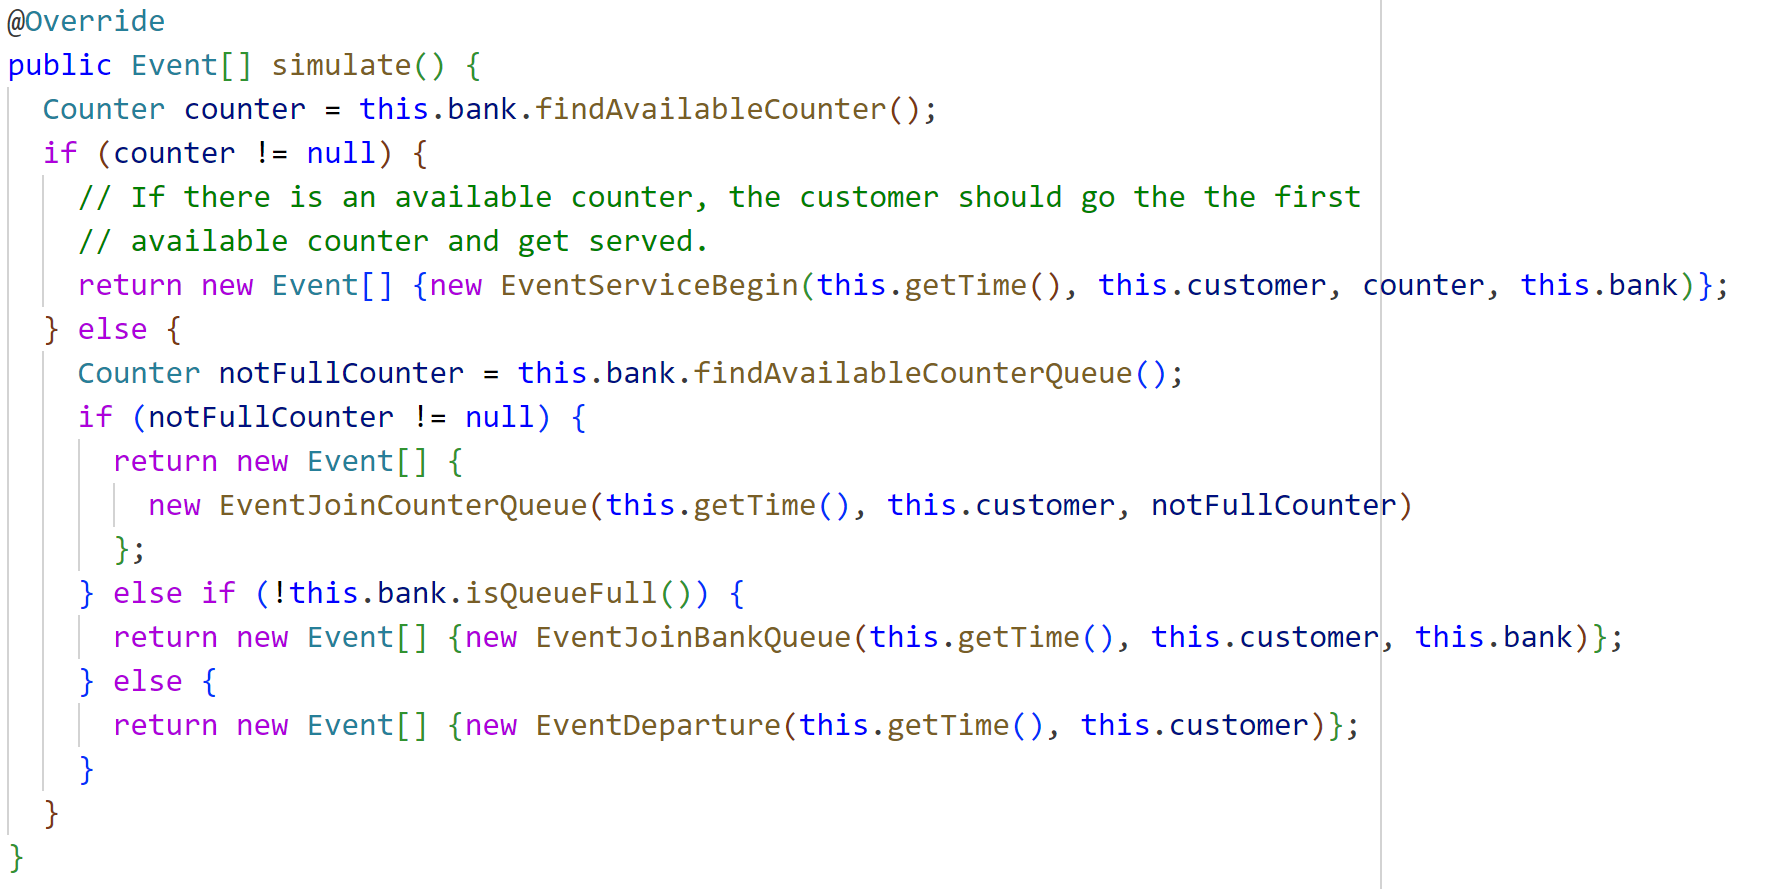
\includegraphics[width=1\linewidth]{PE/PE1/images/PE1-1.png}}
    \textbf{Queue}
    \centerline{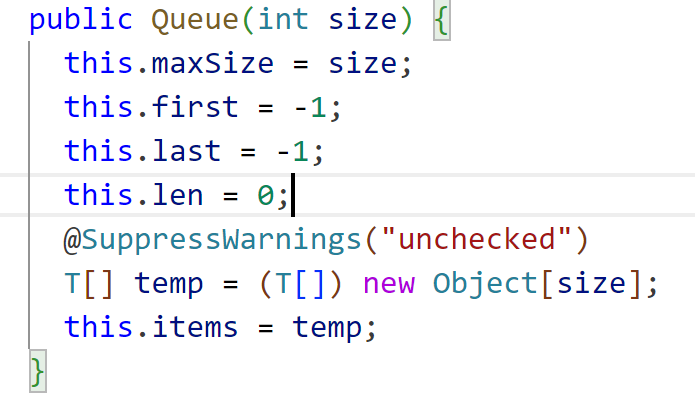
\includegraphics[width=1\linewidth]{PE/PE1/images/PE1-3.png}}
    \textbf{equals design}
    \centerline{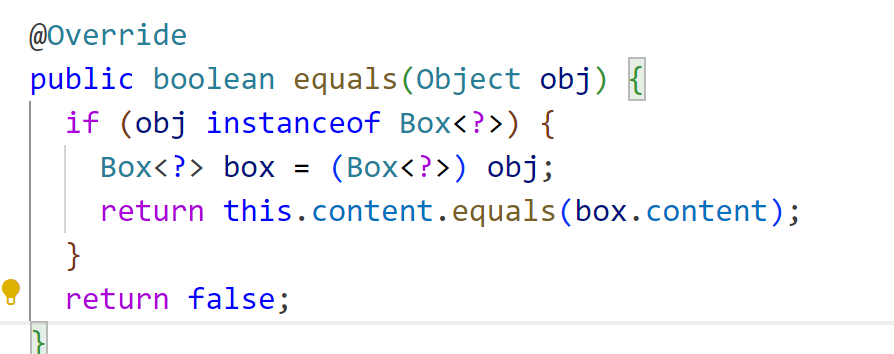
\includegraphics[width=1\linewidth]{PE/PE1/images/PE1-4.png}}
    \textbf{Seq}
    \centerline{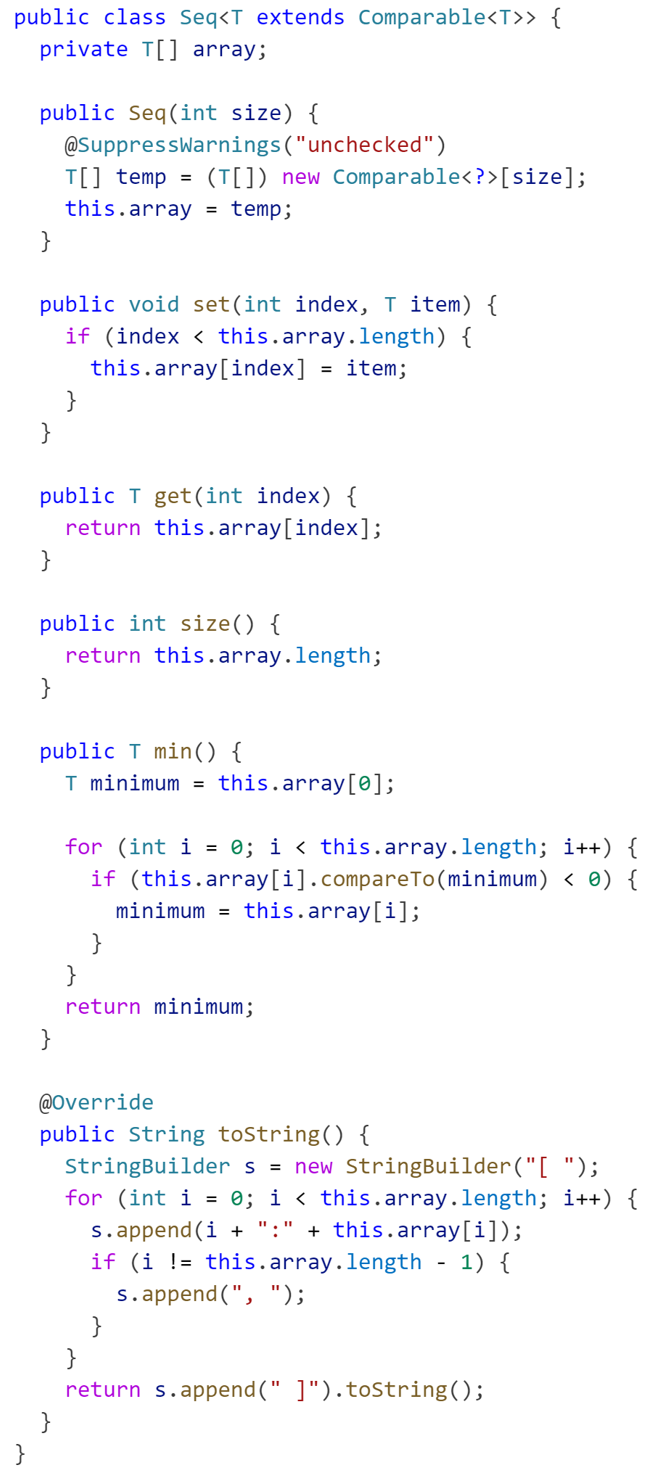
\includegraphics[width=0.75\linewidth]{PE/PE1/images/PE1-2.png}}
    \textbf{Iterate through the Queue}
    \centerline{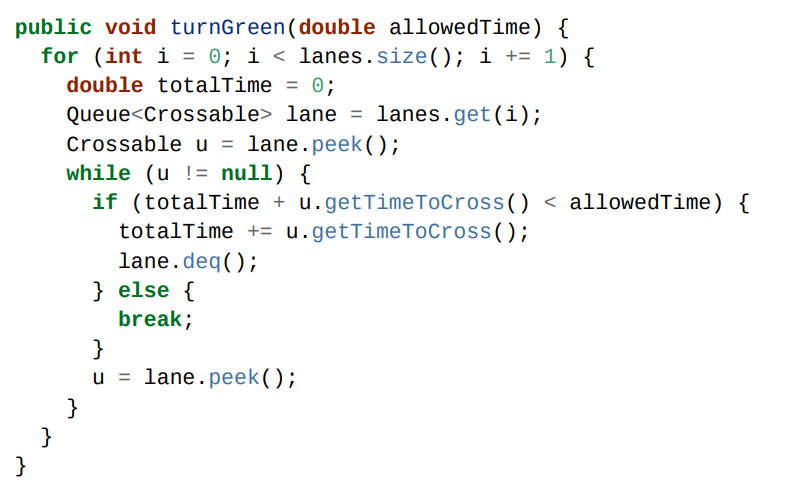
\includegraphics[width=1\linewidth]{PE/PE1/images/PE1-5.png}}

\end{multicols}



\end{document}